\chapter{Project Management}
\label{chap:pm}

As stated throughout \see{chap:methodology}, the Iterative SDLC model was chosen for this project. All tasks will be managed with GitHub projects Kanban, Table and Milestones functionality \see{pm:kanban}. Furthermore, the project will be managed with Git for version control \see{pm:version_control} and regular meetings with the project supervisor were scheduled to monitor progress \see{pm:supervisor_meetings}.

\section{GitHub}

\subsection{Kanban Board and Projects}
\label{pm:kanban}

From the beginning, a GitHub project was created with the code repository to manage all development and writing tasks to be completed \see{fig:kanban}. All tasks were initially added to the backlog and allocated a milestone and label to categorise each task.

\begin{figure}
    \centering
    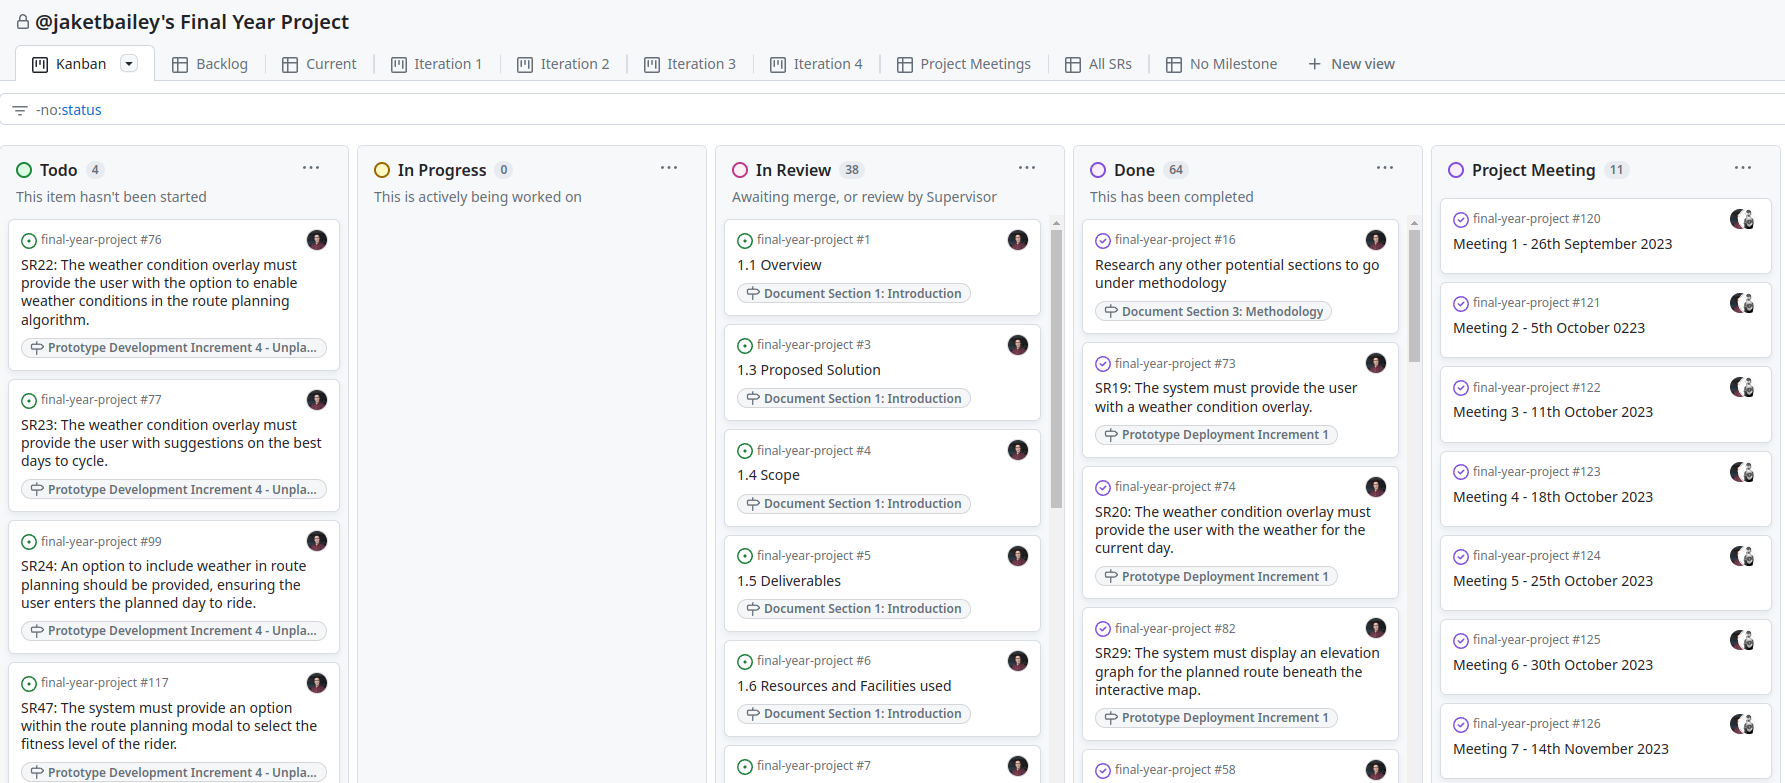
\includegraphics[width=400px]{figures/kanban.png}
    \caption{GitHub Kanban Board}
    \label{fig:kanban}
\end{figure}

Milestones were created for each iteration of the prototype and each section of this document \see{fig:milestones}. Each task would then be assigned a 'To Do' status when selected for development/writing and would progress throughout the other Kanban Board stages until it was marked as 'Done' and closed. This allowed for the effective management of subtasks on a per-milestone and status basis.

\begin{figure}
    \centering
    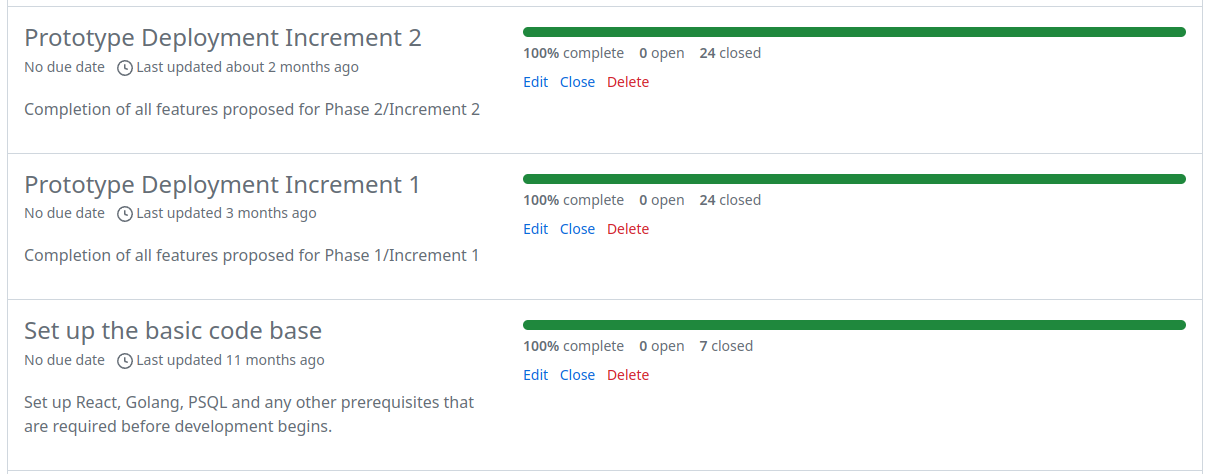
\includegraphics[width=400px]{figures/milestones.png}
    \caption{GitHub Milestones}
    \label{fig:milestones}
\end{figure}

An 'In Review' status was added to the Kanban board for tasks that required guidance from the project supervisor \see{pm:supervisor_meetings}.

\subsection{Version Control}
\label{pm:version_control}

GitHub will host the source code with Git Software Version Management (SVM). Using GitHub and Git enables branches to be created in the repository to manage code changes and link each change to a pull request which enables effective iterative development \see{fig:gitgraph}. Branches allow for branch-level testing and pull requests for automated merges once the increment has been completed. These merges will also throw merge conflicts arise between iterations, ensuring the code base remains accurate, forcing the conflict to be resolved before changes are made. Commits are also highly valuable during development as they allow code changes to be managed and reversed if needed. 

\begin{figure}[!ht]
    \centering
    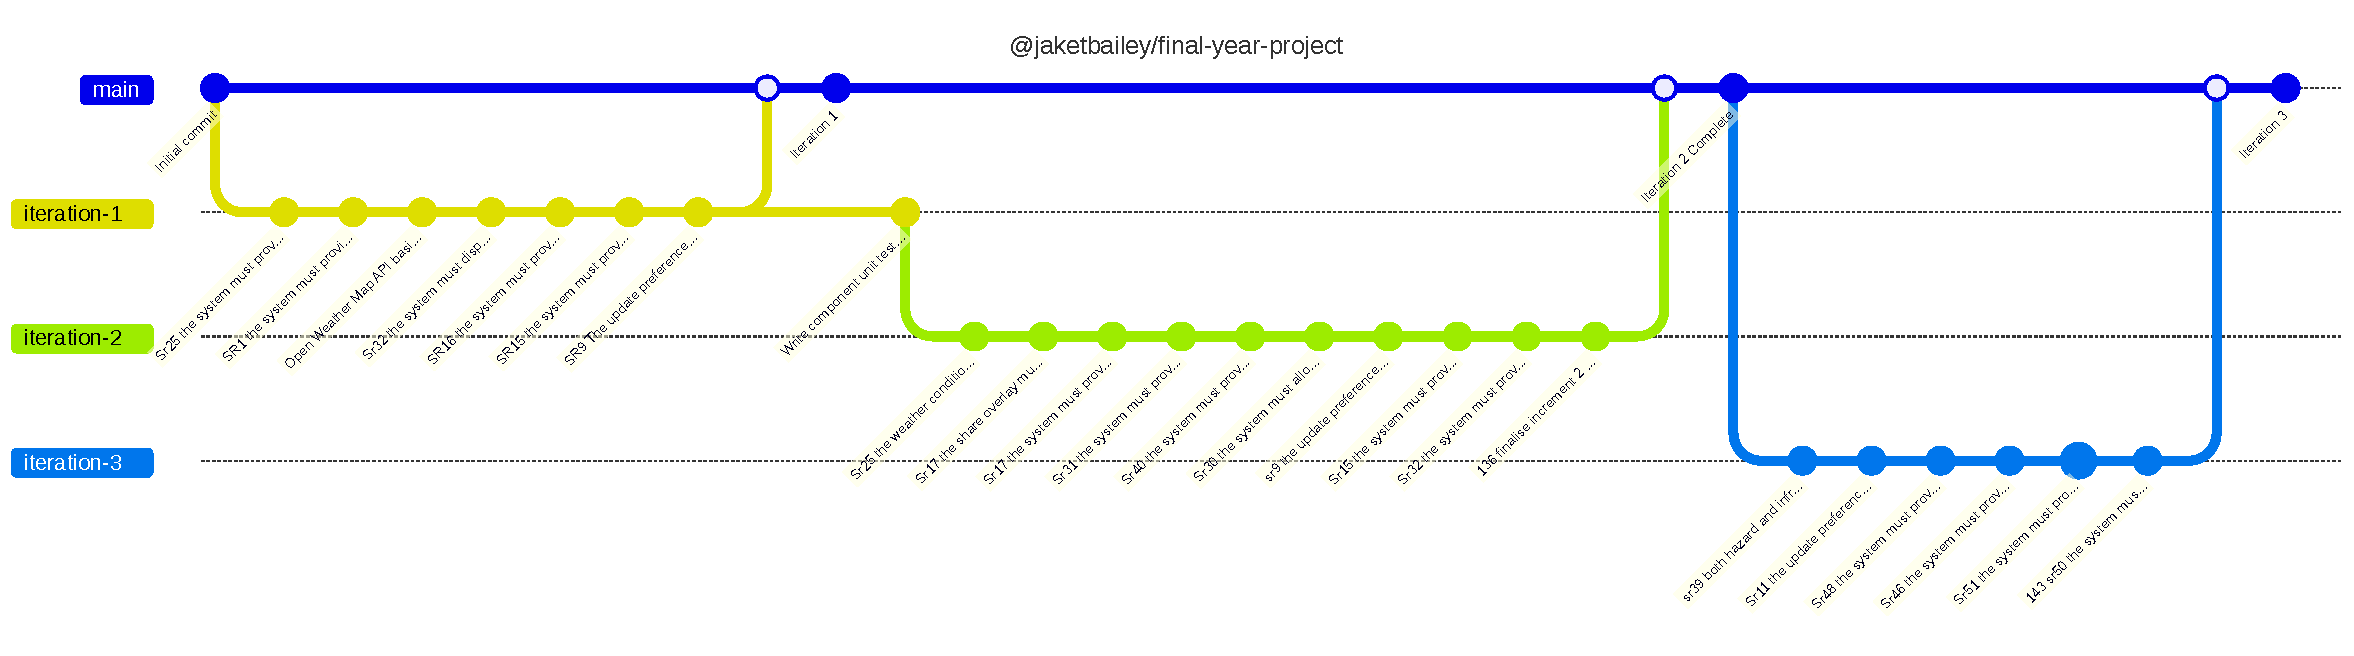
\includegraphics[width=400px]{figures/gitgraph.pdf}
    \caption{Git Pull Requests and Branches}
    \label{fig:gitgraph}
\end{figure}

\section{Supervisor Meetings}
\label{pm:supervisor_meetings}

With the project requiring regular client interaction, regular meetings were scheduled with the supervisor to monitor progress. In-person meetings were preferred, however, due to illness, video conferences were used as a backup. Due to being ahead of schedule, after the 13th meeting, the meetings comprised primarily of project improvements and personal tutor sessions. See the list of meetings below:

\begin{itemize}
    \item \textbf{Meeting 1 - 26th September 2023}
    \begin{itemize}
        \item Discussion of the initial project idea.
        \item Discussion of different approaches to the project.
        \item Discussion of the best way to work with the supervisor.
    \end{itemize}
    \item \textbf{Meeting 2 - 5th October 2023}
    \begin{itemize}
        \item Feedback on initial draft project initiation document.
        \item Outlining overall project objectives.
    \end{itemize}
    \item \textbf{Meeting 3 - 11th October 2023}
    \begin{itemize}
        \item Finalise and submit project initiation document.
        \item Discussion of ethics application.
        \item Discussion of potential primary research methods.
    \end{itemize}
    \item \textbf{Meeting 4 - 18th October 2023}
    \begin{itemize}
        \item Demo and feedback of initial research prototype application.
        \item Demo and feedback of initial basic artefact setup.
        \item Discussion of potential future features.
    \end{itemize}
    \item \textbf{Meeting 5 - 25th October 2023}
    \begin{itemize}
        \item Feedback on document progress so far, working towards literature review.
        \item Discussion on ways to rank and compare feedback from the research application.
    \end{itemize}
    \item \textbf{Meeting 6 - 30th October 2023}
    \begin{itemize}
        \item Feedback on literature review.
        \item Discussion of requirements using research feedback.
    \end{itemize}
    \item \textbf{Meeting 7 - 14th November 2023}
    \begin{itemize}
        \item Feedback on complete literature review.
        \item Feedback and discussion of requirements.
        \item Further discussion of potential future features on top of requirements.
    \end{itemize}
    \item \textbf{Meeting 8 - 29th November 2023}
    \begin{itemize}
        \item Requirements mostly finalised, feedback received.
        \item Discussion on the design of the artefact.
    \end{itemize}
    \item \textbf{Meeting 9 - 8th December 2023}
    \begin{itemize}
        \item Final feedback on project so far for 2023.
        \item Discussion of development/sprint plan for January 2024.
        \item Discussion of plan post-development.
    \end{itemize}
    \item \textbf{Meeting 10 - 10th January 2024}
    \begin{itemize}
        \item Feedback on development progress so far.
        \item Agreement made to delay meetings for 3-4 weeks to allow for development.
        \item Agreement on the plan for post-development (3-4 weeks).
    \end{itemize}
    \item \textbf{Meeting 11 - 9th February 2024}
    \begin{itemize}
        \item Feedback on development
        \item Discussion of end-goal, final artefact/document.
        \item Discussion of the plan for the project stages.
    \end{itemize}
    \item \textbf{Meeting 12 - 16th February 2024}
    \begin{itemize}
        \item Feedback on Design and Implementation chapters.
        \item Agreement on final end goal - 5 weeks from 16th February.
        \item Agreement to complete draft of final document within 2 weeks.
        \item Agreement to use final 3 weeks to review and improve.
        \item Discussion of the use of unplanned extra time (after 5 weeks) to improve artefact.
    \end{itemize}
    \item \textbf{Meeting 13 - 23rd February 2024}
    \begin{itemize}
        \item Guidance provided for last improvements to report.
        \item Discussion on how to use extra time post-easter.
    \end{itemize}
    \item \textbf{Meeting 14 - 28th February 2024}
    \begin{itemize}
        \item Further guidance provided and feedback given on improvements made.
        \item Discussion to build a script to create a Gantt chart from the GitHub repository.
    \end{itemize}
\end{itemize}

\section{Conclusion}
\label{pm:conclusion}

Planning the project management techniques was a key factor when understanding how the requirements in the following chapter would be met. Between the methodology \see{chap:methodology} and project management plan \see{chap:pm}, it was clear how the user stories could be broken down into system requirements, and therefore tasks to complete \see{chap:requirements}. Pre-planning was one of the key successes of the project whereby the project was completed ahead of schedule. Further highlighting how the techniques used influenced the elicited requirements.